\documentclass[a4paper,12pt]{article}

\textwidth 17cm \textheight 25cm \evensidemargin 0cm
\oddsidemargin 0cm \topmargin -2cm
\parindent 0pt
%\parskip \bigskipamount

\usepackage{graphicx}
\usepackage[dutch]{babel}
\usepackage{amssymb,amsthm,amsmath}
%\usepackage{dot2texi}
\usepackage[utf8]{inputenc}
\usepackage{nopageno}
\usepackage{pdfpages}
\usepackage{enumerate}
\usepackage{caption}
\usepackage{wrapfig}
\usepackage{pgf,tikz,pgfplots}
\pgfplotsset{compat=1.15}
\usepackage{color}
\usetikzlibrary{arrows}
\usetikzlibrary{patterns}
\usepackage{fancyhdr}
\pagestyle{fancy}
\usepackage[version=3]{mhchem}
\usepackage{multicol}
\usepackage{fix-cm}
\usepackage{setspace}
\usepackage{mhchem}
\usepackage{xhfill}
\usepackage{parskip}
\usepackage{cancel}
\usepackage{mdframed}
\usepackage{url}
\usepackage{mathtools}
\usepackage{changepage}

\newcommand{\todo}[1]{{\color{red} TODO: #1}}

\newcommand{\degree}{\ensuremath{^\circ}}
\newcommand\rad{\qopname\relax o{\mathrm{rad}}}

\newcommand\ggd{\qopname\relax o{\mathrm{ggd}}}

\pgfmathdeclarefunction{gauss}{2}{%
  \pgfmathparse{1/(#2*sqrt(2*pi))*exp(-((x-#1)^2)/(2*#2^2))}%
}

\def\LRA{\Leftrightarrow}

\newcommand{\zrmbox}{\framebox{\phantom{EXE}}\phantom{X}}
\newcommand{\zrm}[1]{\framebox{#1}}

% environment oefening:
% houdt een teller bij die de oefeningen nummert, probeert ook de oefening op één pagina te houden
\newcounter{noefening}
\setcounter{noefening}{0}
\newenvironment{oefening}
{
  \stepcounter{noefening}
  \pagebreak[0]
  \begin{minipage}{\textwidth}
  \vspace*{0.7cm}{\large\bf Oefening \arabic{noefening}}
}{%
  \end{minipage}
}

\usepackage{calc}

% vraag
\reversemarginpar
\newcounter{punten}
\setcounter{punten}{0}
\newcounter{nvraag}
\setcounter{nvraag}{1}
\newlength{\puntwidth}
\newlength{\boxwidth}
\newcommand{\vraag}[1]{
\settowidth{\puntwidth}{\Large{#1}}
\setlength{\boxwidth}{1.5cm}
\addtolength{\boxwidth}{-\puntwidth}
{\large\bf Vraag \arabic{nvraag} \addtocounter{nvraag}{1}}\vspace*{-0.5cm}
{\marginpar{\color{lightgray}\fbox{\parbox{1.5cm}{\vspace*{1cm}\hspace*{\boxwidth}{\Large{#1}}}}}
\vspace*{0.5cm}}
\addtocounter{punten}{#1}}

% arulefill
\def\arulefill{\leavevmode{\xrfill[-5pt]{0.3pt}[lightgray]\endgraf}\vspace*{0.2cm}}

% \arules{n}
\newcommand{\arules}[1]{
\color{lightgray}
%\vspace*{0.05cm}
\foreach \n in {1,...,#1}{
  \vspace*{0.75cm}
  \hrule height 0.3pt\hfill
}\color{black}\vspace*{0.2cm}}

% \arule{x}
\newcommand{\arule}[1]{
\color{lightgray}{\raisebox{-0.1cm}{\rule[-0.05cm]{#1}{0.3pt}}}\color{black}
}

% \abox{y}
\newcommand{\abox}[1]{
\fbox{
\begin{minipage}{\textwidth- 4\fboxsep}
\hspace*{\textwidth}\vspace{#1}
\end{minipage}
}
}

\newcommand{\ruitjes}[1]{
\definecolor{cqcqcq}{rgb}{0.85,0.85,0.85}
\hspace*{-2.5cm}
\begin{tikzpicture}[scale=1.04,line cap=round,line join=round,>=triangle 45,x=1.0cm,y=1.0cm]
\draw [color=cqcqcq, xstep=0.5cm, ystep=0.5cm] (0,-#1) grid (20.5,0);
\end{tikzpicture}
}


\newcommand{\assenstelsel}[5][1]{
\definecolor{cqcqcq}{rgb}{0.65,0.65,0.65}
\begin{tikzpicture}[line cap=round,line join=round,>=triangle 45,x=#1cm,y=#1cm]
\draw [color=cqcqcq,dash pattern=on 1pt off 1pt, xstep=1.0cm,ystep=1.0cm] (#2,#4) grid (#3,#5);
\draw[->,color=black] (#2,0) -- (#3,0);
%\draw[shift={(1,0)},color=black] (0pt,2pt) -- (0pt,-2pt) node[below] {\footnotesize $1$};
%\draw[color=black] (#3.25,0.07) node [anchor=south west] {$x$};
\draw[->,color=black] (0,#4) -- (0,#5);
%\draw[shift={(0,1)},color=black] (2pt,0pt) -- (-2pt,0pt) node[left] {\footnotesize $1$};
\draw[color=black] (0.09,#5.25) node [anchor=west] {\phantom{$y$}};
%\draw[color=black] (0pt,-10pt) node[right] {\footnotesize $0$};
\end{tikzpicture}
}

\newcommand{\getallenas}[3][1]{
\definecolor{cqcqcq}{rgb}{0.65,0.65,0.65}
\begin{tikzpicture}[scale=#1,line cap=round,line join=round,>=triangle 45,x=1.0cm,y=1.0cm]
\draw [color=cqcqcq,dash pattern=on 1pt off 1pt, xstep=1.0cm,ystep=1.0cm] (#2,-0.2) grid (#3,0.2);
\draw[->,color=black] (#2.25,0) -- (#3.5,0);
\draw[shift={(0,0)},color=black] (0pt,2pt) -- (0pt,-2pt) node[below] {\footnotesize $0$};
\draw[shift={(1,0)},color=black] (0pt,2pt) -- (0pt,-2pt) node[below] {\footnotesize $1$};
\draw[color=black] (#3.25,0.07) node [anchor=south west] {$\mathbb{R}$};
\end{tikzpicture}
}

\newcommand{\visgraad}[1]{\begin{tabular}{p{0.5cm}|p{#1}}&\\\hline\\\end{tabular}}

\newcommand{\tekenschema}[2]{\begin{tabular}{p{0.5cm}|p{#1}}&\\\hline\\[#2]\end{tabular}}

% schema van Horner
\newcommand{\schemahorner}{
\begin{tabular}{p{0.5cm}|p{7cm}}
&\\[1.5cm]
\hline\\
\end{tabular}}

% geef tabular iets meer ruimte
\setlength{\tabcolsep}{14pt}
\renewcommand{\arraystretch}{1.5}

\newcommand{\toets}[3]{
\thispagestyle{plain}
\vspace*{-2.5cm}
\begin{tikzpicture}[remember picture, overlay]
    \node [shift={(15.25 cm,-1.6cm)}] {%
        \includegraphics[width=1.8cm]{/home/ppareit/kaa1415/logokaavelgem.png}%
    };%
\end{tikzpicture}

\begin{tabular}{|llc|c|}
\hline
\vspace*{-0.5cm}
&&&\\
Naam & \arule{4cm} & {\Large\bf KA AVELGEM} & \\
\vspace*{-0.75cm}
&&&\\
Klas & \arule{4cm} & {\Large\bf 20...-...-...} & \\
\hline
\vspace*{-0.75cm}
&&&\\
Toets & {\bf #2} & {\large\bf #1} & Beoordeling\\
\vspace*{-0.75cm}
&&&\\
Onderwerp & \multicolumn{2}{l|}{\bf #3} &\\
\hline
\end{tabular}
}

\newcommand{\oefeningen}[1]{

\fancyhead[LE, RO]{\vspace{0.5cm} #1}
%\thispagestyle{plain}

{\bf \Large \centering Oefeningen: #1}

}

\raggedbottom

\newcommand\vl{\qopname\relax o{\mathrm{vl}}}

\newcommand\dom{\qopname\relax o{\mathrm{dom}}}
\newcommand\ber{\qopname\relax o{\mathrm{ber}}}

\newcommand\mC{\qopname\relax o{\mathrm{mC}}}
\newcommand\uC{\qopname\relax o{\mathrm{{\mu}C}}}
\newcommand\C{\qopname\relax o{\mathrm{C}}}

\newcommand\W{\qopname\relax o{\mathrm{W}}}
\newcommand\kW{\qopname\relax o{\mathrm{kW}}}
\newcommand\kWh{\qopname\relax o{\mathrm{kWh}}}


\newcommand\V{\qopname\relax o{\mathrm{V}}}
\newcommand\ohm{\qopname\relax o{\mathrm{\Omega}}}
\newcommand\kohm{\qopname\relax o{\mathrm{k\Omega}}}


\newcommand\N{\qopname\relax o{\mathrm{N}}}

\newcommand\Nperkg{\qopname\relax o{\mathrm{N/kg}}}

\newcommand\Nperm{\qopname\relax o{\mathrm{N/m}}}

\newcommand\gpermol{\qopname\relax o{\mathrm{g/mol}}}


\newcommand\kgperm{\qopname\relax o{\mathrm{kg/m}}}
\newcommand\kgperdm{\qopname\relax o{\mathrm{kg/dm}}}
\newcommand\gpercm{\qopname\relax o{\mathrm{g/cm}}}
\newcommand\gperml{\qopname\relax o{\mathrm{g/ml}}}


\newcommand{\mA}{\;\mbox{mA}}
\newcommand{\A}{\;\mbox{A}}
\newcommand{\MA}{\;\mbox{MA}}

\newcommand{\us}{\;\mu\mbox{s}}
\newcommand\s{\qopname\relax o{\mathrm{s}}}

\newcommand\h{\qopname\relax o{\mathrm{h}}}

\newcommand{\kmperh}{\;\mbox{km/h}}
\newcommand{\mpers}{\;\mbox{m/s}}
\newcommand{\kmpermin}{\;\mbox{km/min}}
\newcommand{\kmpers}{\;\mbox{km/s}}

\newcommand{\mph}{\;\mbox{mph}}

\newcommand{\Hz}{\;\mbox{Hz}}

\newcommand\Gm{\qopname\relax o{\mathrm{Gm}}}
\newcommand\Mm{\qopname\relax o{\mathrm{Mm}}}
\newcommand\km{\qopname\relax o{\mathrm{km}}}
\newcommand\hm{\qopname\relax o{\mathrm{hm}}}
\newcommand\dam{\qopname\relax o{\mathrm{dam}}}
\newcommand\m{\qopname\relax o{\mathrm{m}}}
\newcommand\dm{\qopname\relax o{\mathrm{dm}}}
\newcommand\cm{\qopname\relax o{\mathrm{cm}}}
\newcommand\mm{\qopname\relax o{\mathrm{mm}}}
\newcommand\um{\qopname\relax o{\mathrm{{\mu}m}}}
\newcommand\nm{\qopname\relax o{\mathrm{nm}}}


\newcommand\Gg{\qopname\relax o{\mathrm{Gg}}}
\newcommand\Mg{\qopname\relax o{\mathrm{Mg}}}
\newcommand\kg{\qopname\relax o{\mathrm{kg}}}
\newcommand\hg{\qopname\relax o{\mathrm{hg}}}
\renewcommand\dag{\qopname\relax o{\mathrm{dag}}}
\newcommand\g{\qopname\relax o{\mathrm{g}}}
\newcommand\dg{\qopname\relax o{\mathrm{dg}}}
\newcommand\cg{\qopname\relax o{\mathrm{cg}}}
\newcommand\mg{\qopname\relax o{\mathrm{mg}}}
\newcommand\ug{\qopname\relax o{\mathrm{{\mu}g}}}
\renewcommand\ng{\qopname\relax o{\mathrm{ng}}}

\newcommand\ton{\qopname\relax o{\mathrm{ton}}}

\newcommand\Gl{\qopname\relax o{\mathrm{Gl}}}
\newcommand\Ml{\qopname\relax o{\mathrm{Ml}}}
\newcommand\kl{\qopname\relax o{\mathrm{kl}}}
\newcommand\hl{\qopname\relax o{\mathrm{hl}}}
\newcommand\dal{\qopname\relax o{\mathrm{dal}}}
\renewcommand\l{\qopname\relax o{\mathrm{l}}}
\newcommand\dl{\qopname\relax o{\mathrm{dl}}}
\newcommand\cl{\qopname\relax o{\mathrm{cl}}}
\newcommand\ml{\qopname\relax o{\mathrm{ml}}}
\newcommand\ul{\qopname\relax o{\mathrm{{\mu}l}}}
\newcommand\nl{\qopname\relax o{\mathrm{nl}}}

\newcommand\MJ{\qopname\relax o{\mathrm{MJ}}}
\newcommand\kJ{\qopname\relax o{\mathrm{kJ}}}
\newcommand\J{\qopname\relax o{\mathrm{J}}}

\newcommand\T{\qopname\relax o{\mathrm{T}}}
\newcommand\uT{\qopname\relax o{\mathrm{{\mu}T}}}

\newcommand\grC{\qopname\relax o{\mathrm{{\degree}C}}}

\newcommand\K{\qopname\relax o{\mathrm{K}}}
\newcommand\calperK{\qopname\relax o{\mathrm{cal/K}}}

\newcommand\hPa{\qopname\relax o{\mathrm{hPa}}}
\newcommand\Pa{\qopname\relax o{\mathrm{Pa}}}

\newcommand\dB{\qopname\relax o{\mathrm{dB}}}

\newcommand\Var{\qopname\relax o{\mathrm{Var}}}

\newcommand{\EE}[1]{\cdot 10^{#1}}

\onehalfspacing

%\setlength{\headsep}{0cm}

\newenvironment{exlist}[1] %
{ \begin{multicols}{#1}
  \begin{enumerate}[(a)]
    \setlength{\itemsep}{0.5em} }
{ \end{enumerate}
  \end{multicols} }




\usepackage{versions}
\includeversion{theorie}


\begin{document}

\pagestyle{fancy}
\lhead{}
\rhead{Oefeningen Goniometrische formules}

\begin{theorie}

\thispagestyle{empty}
\begin{center}
  \begin{mdframed}
  \centering
  \fontsize{40}{50}\selectfont Goniometrische formules
  \end{mdframed}
  \vfill
  \begin{tikzpicture}[scale=5,cap=round,>=latex]
        % draw the coordinates
        \draw[->] (-1.2cm,0cm) -- (1.2cm,0cm) node[right,fill=white] {$x$};
        \draw[->] (0cm,-1.2cm) -- (0cm,1.2cm) node[above,fill=white] {$y$};

        % draw the unit circle
        \draw[line width=1.3pt] (0cm,0cm) circle(1cm);
        \draw[line width=1.6pt, gray] (0cm,0cm) -- (30:1cm);
        \draw[line width=2pt] (0,0) -- ({cos(30)},0);
        \draw[line width=2pt] (0,0) -- (0,{sin(30)});
        \draw[dashed] ({cos(30)},0) -- ({cos(30)},{sin(30)});
        \draw[dashed] (0,{sin(30)}) -- ({cos(30)},{sin(30)});

        \draw (0.25,0.01) node[above=1pt] {$\alpha$};

    \end{tikzpicture}
  \vfill
\end{center}
\subsection*{Doelstelling}
Je \hfill  {\scriptsize(LP 2006-059, LI 1.6.3)}
\begin{itemize}
  \item kan de optellingsformules voor sinus, cosinus en tangens opstellen en toepassen
  \item de verdubbelingsformules voor sinus, cosinus en tangens opstellen en toepassen
  \item de halveringsformules voor sinus en cosinus opstellen en toepassen
  \item de formules van Simpson opstellen en toepassen
\end{itemize}


\pagestyle{empty}
\mbox{}
\newpage
\clearpage
\thispagestyle{empty}
%\mbox{}
\tableofcontents
\newpage
\clearpage
\pagenumbering{arabic}

\pagestyle{fancy}
\lhead{}
\rhead{Goniometrische formules}

\end{theorie}

\onehalfspacing

\section{Goniometrische getallen}

\begin{theorie}

Voor een hoek met maatgetal $\alpha$ en beeldpunt $\vec{p}=(p_x,p_y)$ op de goniometrische cirkel definiëren we de goniometrische getallen als volgt:

\begin{itemize}
  \item De {\bf cosinus} van $\alpha$ is de $x$-coördinaat van $\vec{p}$: $\cos\alpha=p_x$
  \item De {\bf sinus} van $\alpha$ is de $y$-coördinaat van $\vec{p}$: $\cos\alpha=p_y$
\end{itemize}

Merk op:
\begin{itemize}
  \item De goniometrische getallen liggen in het interval $[-1,1]$.
  \item De goniometrische getallen hangen slechts van de hoek af en niet van zijn maatgetal, m.a.w.
  $$\alpha = \alpha + k\cdot 360\degree\mbox{ met }k\in\mathbb{Z}$$
\end{itemize}

Door stelling van Pythagoras toe te passen vinden we de {\bf grondformule van de goniometrie}
$$\cos^2\alpha + \sin^2\alpha = 1$$

Verder worden nog volgende afgeleide goniometrische getallen gedefinieerd:
\begin{itemize}
  \item De {\bf tangens} van $\alpha$:
  $$\tan\alpha=\dfrac{\sin\alpha}{\cos\alpha}$$
  \item De {\bf cotangens} van $\alpha$:
  $$\cot\alpha=\dfrac{\cos\alpha}{\sin\alpha}$$
  \item De {\bf secans} van $\alpha$:
  $$\sec\alpha=\dfrac{1}{\cos\alpha}$$
  \item De {\bf cosecans} van $\alpha$:
  $$\csc\alpha=\dfrac{1}{\cos\alpha}$$
\end{itemize}

\pagebreak
\section{Goniometrische getallen van enkele bijzondere hoeken}
\begin{center}
  \begin{tabular}{c|c|c|c|c|c|c|c|c|c}
    $x$ & $0\degree$ & $30\degree$ & $45\degree$ & $60\degree$ & $90\degree$ & $120\degree$ & $135\degree$ & $150\degree$ & $180\degree$ \\
    \hline
    $\sin x$&&&&&&&&&\\
    \hline
    $\cos x$&&&&&&&&&\\
    \hline
    $\tan x$&&&&&&&&&\\
  \end{tabular}
  \vspace*{0.5cm}\mbox{}
  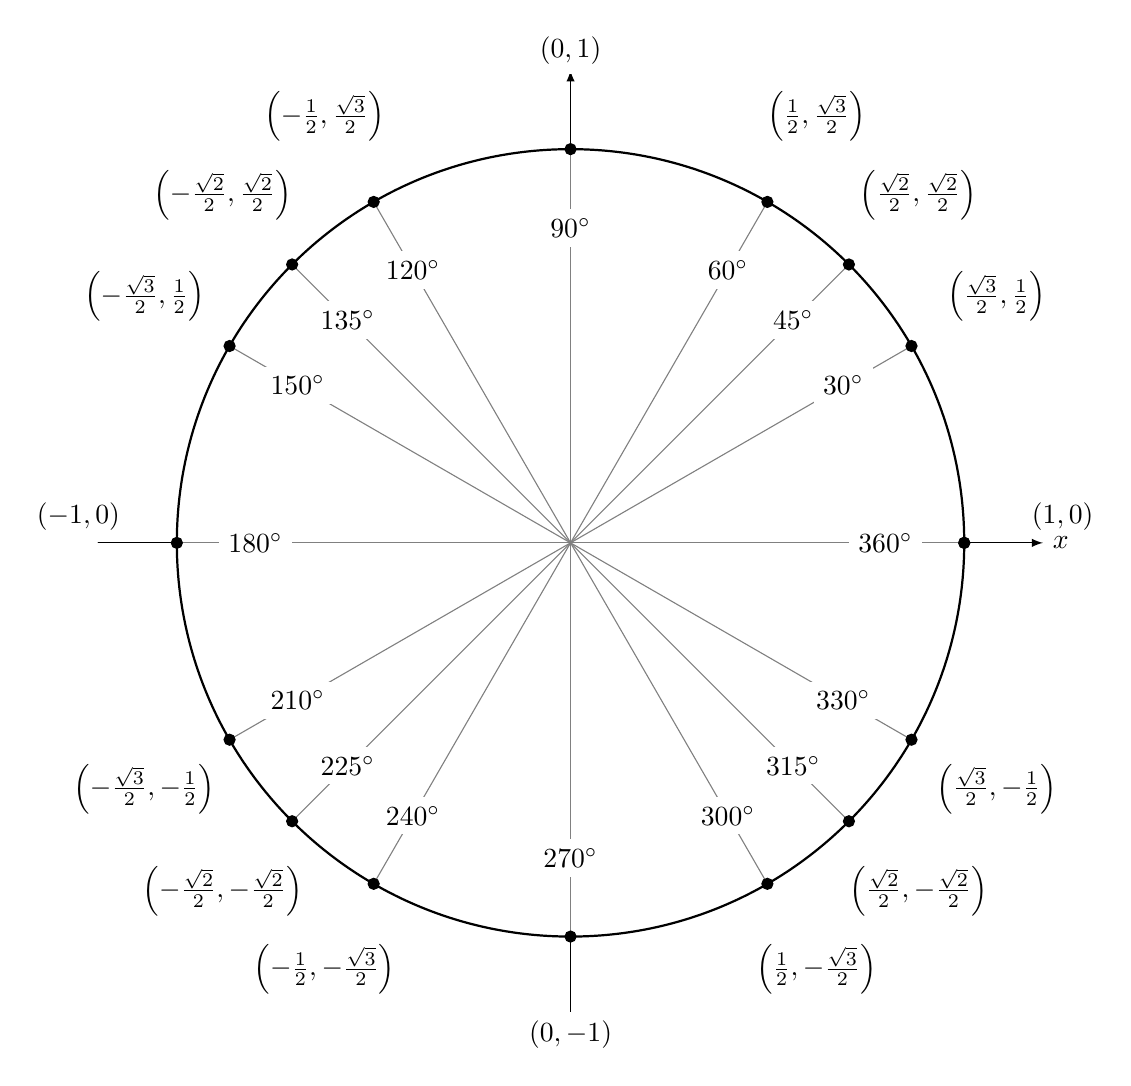
\begin{tikzpicture}[scale=5,cap=round,>=latex]
        % draw the coordinates
        \draw[->] (-1.2cm,0cm) -- (1.2cm,0cm) node[right,fill=white] {$x$};
        \draw[->] (0cm,-1.2cm) -- (0cm,1.2cm) node[above,fill=white] {$y$};

        % draw the unit circle
        \draw[thick] (0cm,0cm) circle(1cm);

        \foreach \x in {0,30,45,60,90,120,135,150,180,210,225,240,270,300,315,330,360} {
                % lines from center to point
                \draw[gray] (0cm,0cm) -- (\x:1cm);
                % dots at each point
                \filldraw[black] (\x:1cm) circle(0.4pt);
                % draw each angle in degrees
                \draw (\x:0.8cm) node[fill=white] {$\x^\circ$};
        }

        \foreach \x/\xtext/\y in {
            % the coordinates for the first quadrant
            30/\frac{\sqrt{3}}{2}/\frac{1}{2},
            45/\frac{\sqrt{2}}{2}/\frac{\sqrt{2}}{2},
            60/\frac{1}{2}/\frac{\sqrt{3}}{2},
            % the coordinates for the second quadrant
            150/-\frac{\sqrt{3}}{2}/\frac{1}{2},
            135/-\frac{\sqrt{2}}{2}/\frac{\sqrt{2}}{2},
            120/-\frac{1}{2}/\frac{\sqrt{3}}{2},
            % the coordinates for the third quadrant
            210/-\frac{\sqrt{3}}{2}/-\frac{1}{2},
            225/-\frac{\sqrt{2}}{2}/-\frac{\sqrt{2}}{2},
            240/-\frac{1}{2}/-\frac{\sqrt{3}}{2},
            % the coordinates for the fourth quadrant
            330/\frac{\sqrt{3}}{2}/-\frac{1}{2},
            315/\frac{\sqrt{2}}{2}/-\frac{\sqrt{2}}{2},
            300/\frac{1}{2}/-\frac{\sqrt{3}}{2}}
                \draw (\x:1.25cm) node[fill=white] {$\left(\xtext,\y\right)$};

        % draw the horizontal and vertical coordinates
        % the placement is better this way
        \draw (-1.25cm,0cm) node[above=1pt] {$(-1,0)$}
              (1.25cm,0cm)  node[above=1pt] {$(1,0)$}
              (0cm,-1.25cm) node[fill=white] {$(0,-1)$}
              (0cm,1.25cm)  node[fill=white] {$(0,1)$};
    \end{tikzpicture}
  \vspace*{0.5cm}
\end{center}

\end{theorie}

\begin{oefening}
Bepaal ook van de andere afgeleide goniometrische getallen, namelijk van cotangens, secans en cosecans ook de waarde van de bijzondere hoeken.
\end{oefening}


\pagebreak
\section{Goniometrische getallen van verwante hoeken}

\begin{theorie}

\subsection{Gelijke hoeken}

\subsubsection*{Definitie}
We noemen twee hoeken $\alpha$ en $\beta$ \textbf{gelijk} als het maatgetal van $\alpha$ gelijk is aan het maatgetal van $\beta$.

\subsubsection*{Geometrische getallen van gelijke hoeken}
Aangezien het maatgetal van een hoek slechts bepaald is op een geheel veelvoud van $360\degree$ zullen gelijke hoeken dezelfde goniometrische getallen hebben.

\subsubsection*{Besluit}
\begin{align*}
\sin(\alpha+k\cdot 360\degree)&=\sin(\alpha)\\
\cos(\alpha+k\cdot 360\degree)&=\cos(\alpha)\\
\tan(\alpha+k\cdot 360\degree)&=\tan(\alpha)\\
\cot(\alpha+k\cdot 360\degree)&=\cot(\alpha)\\
\end{align*}

\end{theorie}

\begin{oefening}
Bereken:
\begin{enumerate}[(a)]
  \item $\sin 390\degree$
  \item $\tan -690\degree$
  \item $\cot -345\degree$
\end{enumerate}
\end{oefening}

\begin{theorie}

\pagebreak
\subsection{Tegengestelde hoeken}
\subsubsection*{Definitie}
We noemen twee hoeken $\alpha$ en $\beta$ \textbf{tegengesteld} als $\alpha=-\beta$.
\subsubsection*{Goniometrische getallen van tegengestelde hoeken}
Teken hieronder een goniometrische cirkel en lees erop af wat het verband is tussen $\sin(\alpha)$ en $\sin(-\alpha)$. Doe hetzelfde voor cos, tan en cot.
\vspace*{7cm}
\subsubsection*{Besluit}
\begin{align*}
  \sin(-\alpha)&=-\sin(\alpha)\\
  \cos(-\alpha)&=\cos(\alpha)\\
  \tan(-\alpha)&=-\tan(\alpha)\\
  \cot(-\alpha)&=-\cot(\alpha)
\end{align*}

\end{theorie}

\begin{oefening}
Bereken
\begin{enumerate}[(a)]
  \item $\sin-45\degree$
  \item $\cos-30\degree$
  \item $\tan-300\degree$
\end{enumerate}
\end{oefening}

\begin{theorie}

\pagebreak
\subsection{Complementaire hoeken}

\subsubsection*{Definitie}
We noemen twee hoeken $\alpha$ en $\beta$ \textbf{complementair} als hun som $90\degree$ is.

\subsubsection*{Goniometrische getallen van complementaire hoeken}
Teken hieronder een goniometrische cirkel en lees erop af wat het verband is tussen $\sin(\alpha)$ en $\sin(90\degree-\alpha)$. Doe hetzelfde voor cos, tan en cot.
\vspace*{7cm}

\subsubsection*{Besluit}
\begin{align*}
  \sin(90\degree-\alpha)&=\cos(\alpha)\\
  \cos(90\degree-\alpha)&=\sin(\alpha)\\
  \tan(90\degree-\alpha)&=\cot(\alpha)\\
  \cot(90\degree-\alpha)&=\tan(\alpha)
\end{align*}

\end{theorie}

\begin{oefening}
Je weet dat de sinus van $20\degree$ ongeveer $0.34$ is, wat is dan de cosinus van $-70\degree$?
\end{oefening}

\begin{theorie}

\pagebreak
\subsection{Supplementaire hoeken}

\subsubsection*{Definitie}
We noemen twee hoeken $\alpha$ en $\beta$ \textbf{supplementair} als hun som $180\degree$ is.

\subsubsection*{Goniometrische getallen van supplementaire hoeken}
Teken hieronder een goniometrische cirkel en lees erop af wat het verband is tussen $\sin(\alpha)$ en $\sin(180\degree-\alpha)$. Doe hetzelfde voor cos, tan en cot.
\vspace*{7cm}
\subsubsection*{Besluit}
\begin{align*}
  \sin(180\degree-\alpha)&=\sin(\alpha)\\
  \cos(180\degree-\alpha)&=-\cos(\alpha)\\
  \tan(180\degree-\alpha)&=-\tan(\alpha)\\
  \cot(180\degree-\alpha)&=-\cot(\alpha)
\end{align*}

\end{theorie}

\begin{oefening}
Bereken
\begin{enumerate}[(a)]
  \item $\sin150\degree$
  \item $\cos135\degree$
  \item $\sin-240\degree$
\end{enumerate}
\end{oefening}

\begin{theorie}

\pagebreak
\subsection{Anti-supplementaire hoeken}

\subsubsection*{Definitie}
We noemen twee hoeken $\alpha$ en $\beta$ \textbf{anti-supplementair} als verschil $180\degree$.

\subsubsection*{Goniometrische getallen van anti-supplementaire hoeken}
Teken hieronder een goniometrische cirkel en lees erop af wat het verband is tussen $\sin(\alpha)$ en $\sin(180\degree+\alpha)$. Doe hetzelfde voor cos, tan en cot.
\vspace*{6cm}

\subsubsection*{Besluit}
\begin{align*}
\sin(180\degree+\alpha)&=-\sin(\alpha)\\
\cos(180\degree+\alpha)&=-\cos(\alpha)\\
\tan(180\degree+\alpha)&=\tan(\alpha)\\
\cot(180\degree+\alpha)&=\cot(\alpha)
\end{align*}

\end{theorie}

\begin{oefening}
Bereken
\begin{enumerate}[(a)]
  \item $\sin210\degree$
  \item $\cos945\degree$
  \item $\sin-120\degree$
\end{enumerate}
\end{oefening}

\begin{theorie}

\pagebreak
\subsection{Oefeningen}

\end{theorie}

\begin{oefening}
Voor de hoek $\alpha$ van $135\degree$
\begin{enumerate}[(a)]
  \item Schets een goniometrische cirkel en duid hierop $\alpha$ aan.
  \item Duid $\sin \alpha$, $\cos \alpha$ en $\cot \alpha$ aan.
  \item Bereken $\sin \alpha$, $\cos \alpha$ en $\cot \alpha$ met behulp van verwante hoeken.
\end{enumerate}
\end{oefening}

\begin{oefening}
Bepaal de waarde van de volgende hoeken:
\begin{enumerate}[(a)]
  \itemsep.5em
  \item $\cos 150\degree$
  \item $\tan 300\degree$
  \item $\sin 315\degree$
  \item $\sec -60\degree$
  \item $\csc -30\degree$
\end{enumerate}
\end{oefening}

\begin{oefening}
Gegeven is dat de volgende vormen zinvol zijn. Schrijf ze zo eenvoudig mogelijk.
\begin{enumerate}[(a)]
  \itemsep1em
  \item $\dfrac{\cos(90\degree-\alpha)}{\tan(180\degree+\alpha)}$
  \item $\dfrac{\sin(90\degree-\alpha)}{\cot(180\degree-\alpha)}$
  \item $\dfrac{\sin(180\degree+\alpha).\tan(180\degree-\alpha)}{\tan(-\alpha)}$
  \item $(1-\cos(-\alpha)).(1+\cos(\alpha))$
  \item $\dfrac{\sin(90\degree-\alpha).\cos(360\degree+\alpha).\cot(90\degree-\alpha)}{\tan(180\degree-\alpha).\cot(\alpha+180\degree).\cos(-\alpha)}$
\end{enumerate}
\end{oefening}

\pagebreak
\section{Optellingsformules}

\begin{theorie}

\subsection{Inleiding}
We willen een formule afleiden om de sinus, cosinus of tangens van een som van twee hoeken te berekenen:
\begin{align*}
  \sin(\alpha + \beta)\\
  \cos(\alpha + \beta)\\
  \tan(\alpha+\beta)
\end{align*}

Vul hiertoe de volgende uitdrukkingen aan en verbind wat aan elkaar gelijk is.

\begin{minipage}{0.4\textwidth}
  $$\sin(30\degree + 60\degree)=\arule{1cm}$$
\end{minipage}
\begin{minipage}{0.5\textwidth}
  $$\sin(30\degree) + \sin(60\degree)=\arule{1cm}$$
  $$\sin(30\degree)\cdot\cos(60\degree)+\cos(30\degree)\cdot\sin(60\degree)=\arule{1cm}$$
\end{minipage}

\begin{minipage}{0.4\textwidth}
  $$\sin(90\degree - 30\degree)=\arule{1cm}$$
\end{minipage}
\begin{minipage}{0.5\textwidth}
  $$\sin(90\degree) + \sin(30\degree)=\arule{1cm}$$
  $$\sin(90\degree)\cdot\cos(30\degree)-\cos(90\degree)\cdot\sin(30\degree)=\arule{1cm}$$
\end{minipage}

\begin{minipage}{0.4\textwidth}
  $$\cos(30\degree + 60\degree)=\arule{1cm}$$
\end{minipage}
\begin{minipage}{0.5\textwidth}
  $$\cos(30\degree) + \cos(60\degree)=\arule{1cm}$$
  $$\cos(30\degree)\cdot\cos(60\degree)-\sin(30\degree)\cdot\sin(60\degree)=\arule{1cm}$$
\end{minipage}

\begin{minipage}{0.4\textwidth}
  $$\cos(90\degree - 30\degree)=\arule{1cm}$$
\end{minipage}
\begin{minipage}{0.5\textwidth}
  $$\cos(90\degree) - \cos(30\degree)=\arule{1cm}$$
  $$\cos(90\degree)\cdot\cos(30\degree)-\sin(90\degree)\cdot\sin(30\degree)=\arule{1cm}$$
\end{minipage}



\subsection{Optellingsformules voor sinus en cosinus}

\subsubsection*{Besluit}
\begin{align*}
  \sin(\alpha + \beta)&=\sin(\alpha)\cdot \cos(\beta)+\cos(\alpha)\cdot \sin(\beta)\\
  \sin(\alpha - \beta)&=\sin(\alpha)\cdot \cos(\beta)-\cos(\alpha)\cdot \sin(\beta)\\
  \cos(\alpha + \beta)&=\cos(\alpha)\cdot \cos(\beta)-\sin(\alpha)\cdot \sin(\beta)\\
  \cos(\alpha - \beta)&=\cos(\alpha)\cdot \cos(\beta)+\sin(\alpha)\cdot \sin(\beta)
\end{align*}


\subsubsection*{Voorbeelden}

\begin{enumerate}[(a)]
  \item Bereken $\sin(75\degree)$
  \vspace*{-0.2cm}
  \begin{align*}
    \sin(75\degree)&=\sin(45\degree+30\degree)\\
                   &=\sin(45\degree+30\degree)\\
                   &=\sin(45\degree)\cdot \cos(30\degree)+\cos(45\degree)\cdot \sin(30\degree)\\
                   &=\frac{\sqrt{2}}{2}\cdot \frac{\sqrt{3}}{2}+\frac{\sqrt{2}}{2}\cdot\frac{\sqrt{1}}{2}\\
                   &=\frac{\sqrt{6}+\sqrt{2}}{4}
  \end{align*}
  \item Bereken $\cos(15\degree)$
  \vspace*{-0.2cm}
  \begin{align*}
    \cos(15\degree)&= \cos(45\degree-30\degree)\\
                   &= \cos 45\degree \cos 30\degree + \sin 45\degree \sin 30\degree\\
                   &= \dfrac{\sqrt{2}}{2}\dfrac{\sqrt{3}}{2} + \dfrac{\sqrt{2}}{2}\dfrac{1}{2}\\
                   &= \dfrac{\sqrt{6} +\sqrt{2}}{4}
  \end{align*}
  \item Vereenvoudig $\cos(4x)\cdot \cos(3x)-\sin(4x)\cdot \sin(3x)$
  \vspace*{-0.2cm}
  \begin{align*}
    \cos(4x)\cdot \cos(3x)-\sin(4x)\cdot \sin(3x)&=\cos(3x+4x)\\
                                                 &=\cos(7x)
  \end{align*}
  \item Vereenvoudig $\cos(19x)\cdot \cos(7x)+\sin(19x)\cdot \sin(7x)$
  \vspace*{-0.2cm}
  \begin{align*}
    \cos(19x)\cdot \cos(7x)+\sin(19x)\cdot \sin(7x)&=\cos(19x-7x)\\
                                                 &=\cos(12x)
  \end{align*}
\end{enumerate}

\pagebreak
\subsection{Optellingsformules voor tangens}
Uitgaande van deze formules leiden we nu een formule af voor de tangens van een som van 2 hoeken.

\subsubsection*{Opstellen formule}
\begin{align*}
  \tan(\alpha + \beta) &= \dfrac{\sin(\alpha + \beta)}{\cos(\alpha+\beta)}\\
                       &= \dfrac{\sin(\alpha)\cdot \cos(\beta)+\cos(\alpha)\cdot \sin(\beta)}{\cos(\alpha)\cdot \cos(\beta)-\sin(\alpha)\cdot \sin(\beta)}\\
                       &= \dfrac{\dfrac{\sin\alpha\cdot\cos\beta}{\cos\alpha\cdot\cos\beta}+\dfrac{\cos\alpha\cdot\sin\beta}{\cos\alpha\cdot\cos\beta}}{\dfrac{\cos\alpha\cdot\cos\beta}{\cos\alpha\cdot\cos\beta}+\dfrac{\sin\alpha\cdot\sin\beta}{\cos\alpha\cdot\cos\beta}}\\
                       &= \dfrac{\tan\alpha+\tan\beta}{1-\tan\alpha\cdot\tan\beta}
\end{align*}

In deze formule moeten $\alpha\neq 90\degree + k\cdot 180\degree$ en $\beta \neq 90\degree + k\cdot 180\degree$ teneinde te beletten dat $\tan\alpha$ en $\tan\beta$ niet zouden bestaan!

We spreken af om enkel hoeken te gebruiken waarvoor de gegeven vormen zinvol zijn. Er geldt ook:
\begin{align*}
  \tan(\alpha - \beta) &= \tan(\alpha + (-\beta))\\
                       &= \dfrac{\tan\alpha + \tan(-\beta)}{1-\tan\alpha\cdot\tan(-\beta)}\\
                       &= \dfrac{\tan\alpha - \tan\beta}{1+\tan\alpha\cdot\tan\beta}
\end{align*}

\subsubsection*{Besluit}
\begin{align*}
  \tan(\alpha + \beta)&=\frac{\tan(\alpha)+\tan(\beta)}{1-\tan(\alpha)\cdot\tan(\beta)}\\
  \tan(\alpha - \beta)&=\frac{\tan(\alpha)-\tan(\beta)}{1+\tan(\alpha)\cdot\tan(\beta)}
\end{align*}

\pagebreak
\subsubsection*{Voorbeelden}
Bereken
\begin{enumerate}[(a)]
  \item $\tan(60\degree - 30\degree)$
  \vspace*{-0.5cm}
  \begin{align*}
    \tan(60\degree - 30\degree)&=\dfrac{\tan(60\degree)-\tan(30\degree)}{1+\tan(60\degree)\cdot\tan(30\degree)}\\
                               &=\dfrac{\sqrt{3}-\frac{\sqrt{3}}{3}}{1+\sqrt{3}\cdot\frac{\sqrt{3}}{3}}\\
                               &=\dfrac{\frac{2}{3}\cdot\sqrt{3}}{2}\\
                               &=\dfrac{\sqrt{3}}{3}
  \end{align*}
  \item $\tan(75\degree)$
  \vspace*{-0.5cm}
  \begin{align*}
    \tan(75\degree) &= \tan(45\degree + 30\degree)\\
                    &= \dfrac{\tan45\degree+\tan30\degree}{1-\tan45\degree\cdot\tan30\degree}\\
                    &= \dfrac{1+\frac{\sqrt{3}}{3}}{1-1\cdot\frac{\sqrt{3}}{3}}\\
                    &= \ldots\\
                    &= 2+\sqrt{3}
  \end{align*}
\end{enumerate}


\subsection{Oefeningen}

\end{theorie}

\begin{oefening}
Bereken
\begin{multicols}{3}
\begin{enumerate}[(a)]
  \item $\cos(75\degree)$
  \item $\sin(15\degree)$
  \item $\tan(105\degree)$
\end{enumerate}
\end{multicols}
\end{oefening}

\begin{oefening}
Vereenvoudig
\begin{enumerate}[(a)]
  \itemsep.5em
  \item $\sin\frac{2x}{3}\cdot \cos\frac{x}{6}-\cos\frac{2x}{3}\cdot \sin\frac{x}{6}$
  \item $\cos\frac{8x}{5}\cdot \cos\frac{x}{10}+\sin\frac{8x}{5}\cdot \sin\frac{x}{10}$
  \item $\cos(110\degree)\cdot \cos(50\degree)+\sin(110\degree)\cdot \sin(50\degree)$
  \item $\sin(72\degree)\cdot \cos(27\degree)-\cos(72\degree)\cdot \sin(27\degree)$
\end{enumerate}
\end{oefening}

\begin{oefening} % got list from Iris, source unknown
Bewijs
\begin{enumerate}[(a)]
  \itemsep.5em
  \item $\displaystyle \cot(\alpha+\beta)=\dfrac{\cot\alpha\cdot\cot\beta-1}{\cot\alpha+\cot\beta}$
  \item $\displaystyle \cos(\alpha-\beta)+\cos(\alpha+\beta)=2\cos\alpha\cos\beta$
  \item $\displaystyle \cos(\alpha-\beta)-\cos(\alpha+\beta)=2\sin\alpha\sin\beta$
  \item $\displaystyle (\sin\alpha + \cos\alpha)(\sin\beta + \cos\beta)=\sin(\alpha+\beta) + \cos(\alpha-\beta)$
  \item $\displaystyle \cos(\alpha + \beta)\cdot\cos(\alpha - \beta) = 1 - \sin^2\alpha - \sin^2\beta$
  \item $\displaystyle \cos(60\degree - \alpha) + \cos(60\degree + \alpha) = \cos\alpha$
  \item $\displaystyle \sin(\alpha + 30\degree) - \sin(\alpha - 30\degree)=\cos\alpha$
  \item $\displaystyle \sin^2(45\degree + \alpha) = \dfrac{1}{2} + \sin\alpha\cos\alpha$
  \item $\displaystyle \cos^2\alpha + \cos^2(120\degree + \alpha)+\cos^2(120\degree - \alpha)=\dfrac{3}{2}$
  \item $\displaystyle \tan(60\degree + \alpha)\cdot\cot(30\degree + \alpha) = \dfrac{3 - \tan^2\alpha}{1-3\tan^2\alpha}$
  \item $\displaystyle \dfrac{\tan(\alpha-\beta) + \tan\beta}{1 - \tan(\alpha - \beta)\cdot\tan\beta} = \tan\alpha$
  \item $\displaystyle \dfrac{\sin(x-y)}{\cos x \cos y} + \dfrac{\sin(y-z)}{\cos y \cos z} + \dfrac{\sin(z-x)}{\cos z \cos x} = 0$
  \item $\displaystyle \tan^2 x - \tan^2 y = \dfrac{\sin(x+y)\cdot\sin(x-y)}{\cos^2 x \cos^2 y}$
  \item $\displaystyle (\cos x + \cos y)^2 + (\sin x - \sin y)^2 = 2 + 2\cos(x+y)$
  \item $\displaystyle \dfrac{\sin(\alpha + \beta)}{\cos(\alpha - \beta)} = \dfrac{\tan \alpha + \tan \beta}{1 + \tan\alpha \tan\beta}$
\end{enumerate}
\end{oefening}

\pagebreak
\section{Verdubbelingsformules}

\begin{theorie}

\subsection{Inleiding}
Is $\sin(2\alpha)$ gelijk aan $2\sin\alpha$?

Probeer het eens met bijvoorbeeld $\alpha=30\degree$?

\begin{minipage}{0.3\textwidth}
\begin{align*}
  \sin(2\cdot30\degree) &= \sin 60\degree\\
                        &= \dfrac{\sqrt{3}}{2}
\end{align*}
\end{minipage}
\begin{minipage}{0.3\textwidth}
\begin{align*}
  2\cdot\sin(30\degree) &= 2\cdot\dfrac{1}{2}\\
                        &= 1
\end{align*}
\end{minipage}

Als we een hoek verdubbelen betekent dit niet dat de sinus, cosinus of tangens van deze hoek ook verdubbeld wordt!

\subsection{Formules voor $\sin 2\alpha$ en $\cos 2\alpha$}

%\subsubsection*{Opstellen formules}

Stellen we $\beta=\alpha$ in de optellingsformule $\sin(\alpha+\beta)=\sin\alpha\cdot\cos\beta + \cos\alpha\cdot\sin\beta$ dan krijgen we
\begin{align*}
       && \sin 2\alpha &= \sin\alpha\cdot\cos\alpha+\cos\alpha\cdot\sin\alpha\\
  \LRA && \sin 2\alpha &= 2\cdot\sin\alpha\cdot\cos\alpha
\end{align*}

Stellen we $\beta=\alpha$ in de optellingsformule $\cos(\alpha+\beta)=\cos\alpha\cdot\cos\beta + \sin\alpha\cdot\sin\beta$ dan krijgen we
\begin{align*}
       && \cos 2\alpha &= \cos\alpha\cdot\cos\alpha+\sin\alpha\cdot\sin\alpha\\
  \LRA && \cos 2\alpha &= \cos^2\alpha -\sin^2\alpha
\end{align*}

Het blijkt dus dat voor het berekenen van $\sin 2\alpha$ of $\cos 2\alpha$ zowel $\sin\alpha$ als $\cos\alpha$
nodig is. Vermits $\sin^2\alpha + \cos^2\alpha = 1$ volstaat echter de kennis van of $\sin\alpha$ of
$\cos\alpha$. Vooral bij $\cos 2\alpha$ wordt dit vaak toegepast:
\begin{align*}
       \cos 2\alpha &= \cos^2\alpha - \sin^2\alpha\\
                    &= (1 - \sin^2\alpha) - \sin^2\alpha\\
                    &= 1 - 2\sin^2\alpha
\end{align*}
\begin{align*}
       \cos 2\alpha &= \cos^2\alpha - \sin^2\alpha\\
                    &= \cos^2\alpha - (1 - \cos^2\alpha)\\
                    &= 2\cos^2\alpha - 1
\end{align*}

\subsubsection*{Besluit}
\begin{align*}
  \sin 2\alpha &= 2\cdot\sin\alpha\cdot\cos\alpha\\
  \cos 2\alpha &= \cos^2\alpha -\sin^2\alpha\\
  \cos 2\alpha &= 1 - 2\sin^2\alpha\\
  \cos 2\alpha &= 2\cos^2\alpha - 1\\
\end{align*}
En ook
\begin{align*}
  1 - \cos 2\alpha &= 2\sin^2\alpha\\
  1 + \cos 2\alpha &= 2\cos^2\alpha \\
\end{align*}

\subsubsection*{Voorbeelden}
\begin{enumerate}[(a)]
  \item Bepaal $\sin 2\alpha$ en $\cos 2\alpha$ als je weet dat $\alpha$ in het eerste kwadrant ligt en als er geldt dat $\cos\alpha=\dfrac{1}{3}$.
    $$\cos 2\alpha = 2\cos^2\alpha - 1 = 2\cdot \dfrac{1}{9}-1=-\dfrac{7}{9}$$
    \begin{align*}
           && \cos^2 2\alpha + \sin^2 2\alpha &= 1\\
      \LRA &&                  \sin^2 2\alpha &= 1 - \cos^2 2\alpha\\
      \LRA &&                  \sin 2\alpha   &= \sqrt{1 - \cos^2 2\alpha}\\
           &&                                 &= + \sqrt{1 - \dfrac{49}{81}}\\
           &&                                 &= \dfrac{4}{9}\cdot\sqrt{2}
    \end{align*}
    Merk op dat gegeven is dat $\alpha\in\mbox{I}$ ligt, dus $2\alpha\in\mbox{I of II}$, dus $\sin 2\alpha$ is positief, vandaar de $+$ voor de wortel.
    \item Bewijs $(\cos \alpha + \sin \alpha + 1)\cdot(\cos\alpha + \sin\alpha - 1)=\sin 2\alpha$
    \begin{align*}
      \mbox{LL} &= (\cos\alpha + \sin\alpha)^2 - 1^2\\
                &= \underbrace{\cos^2\alpha + \sin^2\alpha}_1 + 2\cos\alpha\cdot\sin\alpha - 1\\
                &= 2\cos\alpha\cdot\sin\alpha\\
                &= \sin 2\alpha = \mbox{RL}
    \end{align*}
\end{enumerate}

\end{theorie}

\begin{oefening}
Bepaal $\sin 2\alpha$ en $\cos 2\alpha$ als je weet dat $\alpha$ in het derde kwadrant ligt en als er geldt dat $\sin\alpha=-\dfrac{1}{4}$ is.
\end{oefening}

\begin{oefening} % list from Iris, source unknown
Bewijs:
\begin{enumerate}[(a)]
  \itemsep.5em
  \item $\displaystyle 4(\cos^6\alpha-\sin^6\alpha)=\cos 2\alpha \cdot(4 - \sin^2 2\alpha)$
  \item $\displaystyle \dfrac{1-\sin 2\alpha}{\cos 2\alpha}=\dfrac{1-\tan\alpha}{1+\tan\alpha}$
  \item $\displaystyle \sin 2x = \dfrac{2}{\tan x + \cot x}$
  \item $\displaystyle \cos 2x = \dfrac{\cot x - \tan x}{\cot x + \tan x}$
  \item $\displaystyle \dfrac{2x}{1+\cos 2x} = \tan x$
  \item $\displaystyle \dfrac{\cos^3 x + \sin^3 x}{\cos x + \sin x} = 1 - \dfrac{1}{2}\sin 2x$
  \item $\displaystyle \dfrac{1}{\sin 2x} + \cot 2x = \cot x$
  \item $\displaystyle \dfrac{1 + \tan^2x}{1 - \tan^2x} = \dfrac{1}{\cos 2x}$
  \item $\displaystyle \dfrac{1}{\cos 2x} = \dfrac{\dfrac{1}{\sin^2x}}{\quad\dfrac{1}{\sin^2x}-2\quad}$
\end{enumerate}
\end{oefening}

\begin{theorie}

\subsection{Formule voor $\tan 2\alpha$}

Stellen we $\beta=\alpha$ in $\tan(\alpha + \beta)=\dfrac{\tan\alpha + \tan\beta}{1-\tan\alpha\cdot\tan\beta}$ dan krijgen we
$$\tan 2\alpha = \dfrac{2\cdot \tan\alpha}{1-\tan^2\alpha}$$

\subsubsection*{Voorbeeld}

Te bewijzen: $\tan\alpha = \dfrac{1}{\sin 2\alpha} - \cot 2\alpha$\\
Bewijs:
\begin{align*}
  \mbox{RL} &= \dfrac{1}{2\sin\alpha \cos\alpha}-\dfrac{1-\tan^2\alpha}{2\tan\alpha}\\
            &= \dfrac{1}{2\sin\alpha \cos\alpha}-\dfrac{1-\dfrac{\sin^2\alpha}{\cos^2\alpha}}{2\cdot \dfrac{\sin\alpha}{\cos\alpha}}\\
            &= \dfrac{1}{2\sin\alpha \cos\alpha}-\dfrac{\cos^2\alpha - \sin^2\alpha}{2\sin\alpha\cos\alpha}\\
            &= \dfrac{1 - \cos^2\alpha + \sin^2\alpha}{2\sin\alpha \cos\alpha}\\
            &= \dfrac{2\sin^2\alpha}{2\sin\alpha \cos\alpha}\\
            &= \dfrac{\sin\alpha}{\cos\alpha} = \mbox{LL}\\
\end{align*}

\end{theorie}

\begin{oefening} % list from Iris, source unknown
Bewijs:
\begin{enumerate}[(a)]
  \itemsep.5em
  \item $\displaystyle \tan^2\alpha\cdot\tan 2\alpha=\tan 2\alpha - 2\tan\alpha$
  \item $\displaystyle \cot x - \tan x = 2\cdot\cot 2x$
  \item $\displaystyle \tan 2x + \dfrac{1}{\cos 2x} = \dfrac{\cos x + \sin x}{\cos x - \sin x}$
\end{enumerate}
\end{oefening}

\begin{theorie}

\subsection{Vervangen van $2\alpha$ door $\alpha$}

Aangezien voorgaande formules werden opgesteld onverschillig van de ligging van de
beeldpunten van de beschouwde georiënteerde hoeken op de goniometrische cirkel,
mag men in die formules $2\alpha$ vervangen door $\alpha$ op voorwaarde dat ook
$\alpha$ door $\dfrac{\alpha}{2}$ wordt vervangen.

\subsubsection*{Voorbeelden}
\begin{itemize}
  \item $\sin\alpha = 2\cdot\sin\dfrac{\alpha}{2}\cdot\cos\dfrac{\alpha}{2}$
  \item $\cos\alpha = \cos^2\dfrac{\alpha}{2}-\sin^2\dfrac{\alpha}{2}$
\end{itemize}

\end{theorie}

\begin{oefening}
Bewijs:
$$\dfrac{\cos\dfrac{\alpha}{2}-\sin\dfrac{\alpha}{2}}{\sin\dfrac{\alpha}{2}+\cos\dfrac{\alpha}{2}}=\dfrac{1-\sin\alpha}{\cos\alpha}$$
\end{oefening}

\begin{theorie}

\subsection{Formules voor $3\alpha$}

Doordat $3\alpha=2\alpha + \alpha$ kan men volgende formules mits enig werk ook afleiden:
\begin{align*}
  \sin 3\alpha &= 3\sin\alpha -4\sin^3\alpha\\
  \cos 3\alpha &= 4\cos^3\alpha -3\cos\alpha\\
  \tan 3\alpha &= \dfrac{3\tan\alpha -\tan^3\alpha}{1-3\tan^2\alpha}
\end{align*}

\pagebreak
\section{Halveringsformules en $t$-formules}

\vspace*{-0.5cm}
\subsection{Inleiding}
Hebben we in het voorgaande hoofdstuk de hoek verdubbeld en formules opgesteld
voor $\sin 2\alpha$, $\cos 2\alpha$ en $\tan 2\alpha$ dan vraagt men ons ditmaal de hoek te halveren .

\vspace*{-0.5cm}
\subsection{Halveringsformules}

We hernemen de verdubbelingsformules voor de cosinus
\begin{align*}
  \cos 2\alpha &= 1 - 2\sin^2\alpha\\
  \cos 2\alpha &= 2\cos^2\alpha - 1
\end{align*}
en vervangen $2\alpha$ door $\alpha$ en $\alpha$ door $\dfrac{\alpha}{2}$ en krijgen
\begin{align*}
  \cos \alpha &= 1 - 2\sin^2\dfrac{\alpha}{2}\\
  \cos \alpha &= 2\cos^2\dfrac{\alpha}{2} - 1\;.
\end{align*}
Uit de eerste formule leiden we $\sin\dfrac{\alpha}{2}$ af uitgedrukt in $\cos\alpha$:
\begin{align*}
          && \sin^2\dfrac{\alpha}{2} &= \dfrac{1-\cos\alpha}{2}\\
     \LRA &&   \sin\dfrac{\alpha}{2} &= +\sqrt{\dfrac{1-\cos\alpha}{2}} \mbox{ of } \sin\dfrac{\alpha}{2}= -\sqrt{\dfrac{1-\cos\alpha}{2}}
\end{align*}

Uit de tweede formule leiden we $\cos\dfrac{\alpha}{2}$ af uitgedrukt in $\cos\alpha$:
\begin{align*}
          && \cos^2\dfrac{\alpha}{2} &= \dfrac{1+\cos\alpha}{2}\\
     \LRA &&   \cos\dfrac{\alpha}{2} &= +\sqrt{\dfrac{1+\cos\alpha}{2}} \mbox{ of } \sin\dfrac{\alpha}{2}= -\sqrt{\dfrac{1+\cos\alpha}{2}}
\end{align*}
Het teken vóór de vierkantswortel wordt bepaald door het kwadrant waarin het
beeldpunt van de georiënteerde hoek met maatgetal $\dfrac{\alpha}{2}$ valt.

Door lid aan lid te delen bekomen we ook nog de halveringsformule voor de tangens
$$\tan\dfrac{\alpha}{2} = +\sqrt{\dfrac{1-\cos\alpha}{1+\cos\alpha}} \mbox{ of } \tan\dfrac{\alpha}{2} = -\sqrt{\dfrac{1-\cos\alpha}{1+\cos\alpha}}$$

Al deze formules hebben het nadeel {\em irrationaal} te zijn, ze bevatten een vierkantswortel in het rechterlid.
Daarom doen we liever een beroep op de volgende formules.

\subsection{$t$-formules}

We leiden de $t$-formule voor sinus af:

\begin{align*}
  \left\{\begin{aligned}\sin 2\alpha = 2\sin\alpha\cos\alpha\\\sin^2\alpha + \cos^2\alpha = 1\end{aligned}\right. \quad
  &\LRA\quad \sin 2\alpha = \dfrac{2\sin\alpha\cos\alpha}{\sin^2\alpha + \cos^2\alpha}\\
  &\LRA\quad \sin 2\alpha = \dfrac{2\dfrac{\sin\alpha}{\cos\alpha}}{\dfrac{\sin^2\alpha}{\cos^2\alpha}+1}\\
  &\LRA\quad \sin 2\alpha = \dfrac{2\tan\alpha}{1+\tan^2\alpha}
\end{align*}

We vervangen terug $2\alpha$ door $\alpha$ en dus ook $\alpha$ door $\dfrac{\alpha}{2}$ en krijgen dan
$$\sin\alpha = \dfrac{2\tan\dfrac{\alpha}{2}}{1+\tan^2\dfrac{\alpha}{2}}$$

Stellen we nu $\tan\dfrac{\alpha}{2}=t$ dan krijgen we
$$\sin\alpha = \dfrac{2t}{1+t^2}$$

Analoog voor cosinus en tangens.

\subsubsection*{Besluit}
\begin{align*}
  \sin\alpha &= \dfrac{2t}{1+t^2}\\
  \cos\alpha &= \dfrac{1-t^2}{1+t^2}\\
  \tan\alpha &= \dfrac{2t}{1-t^2}
\end{align*}
met $t=\tan \dfrac{\alpha}{2}$.

\end{theorie}

\begin{oefening}
Bewijs zelf de $t$-formules voor cosinus en tangens.
\end{oefening}

\begin{theorie}

\subsection{Oefeningen}

\end{theorie}

\begin{oefening}
Bepaal $\sin\alpha$, $\cos\alpha$ en $\tan\alpha$ als gegeven is dat $\tan\dfrac{\alpha}{2}=2+\sqrt{3}$.
\end{oefening}

\begin{oefening}
Bereken $\tan\dfrac{\alpha}{2}$ als $\sqrt{3}\cdot\sin\alpha+\cos\alpha=1$.
\end{oefening}

\begin{oefening}
Bewijs
$$\cos\alpha=\dfrac{1}{1+\tan\alpha\cdot\tan\dfrac{\alpha}{2}}\;.$$
\end{oefening}

\begin{oefening}
Bepaal $\tan\dfrac{\alpha}{2}$ als $\cos\beta\cdot\sin\alpha+\tan\gamma\cdot\alpha=\tan\gamma\cdot\sin\beta$.
\end{oefening}


\newpage
\section{Formules van Simpson}

\begin{theorie}

\subsection{Inleiding}

Uit de optellingsformules kunnen we formules afleiden die een product van
sinussen en/of cosinussen omzetten in een som en omgekeerd.

Bepaalde toepassingen later eisen factoren (bij vermenigvuldiging) in plaats van
termen (bij optelling) of vice versa.

Deze formules zullen je toelaten van de ene naar de andere vorm over te stappen.

\subsection{Eerste vorm van de formules van Simpson: product omzetten naar som}

\subsubsection*{Opstellen formules}

We vertrekken vanuit de optellingsformules
\begin{align*}
                   \sin(\alpha + \beta) &= \sin\alpha\cdot\cos\beta + \cos\alpha\cdot\sin\beta\\
  \mbox{en }\qquad \sin(\alpha - \beta) &= \sin\alpha\cdot\cos\beta - \cos\alpha\cdot\sin\beta
\end{align*}

Lid aan lid optellen geeft
$$\sin(\alpha+\beta) + \sin(\alpha - \beta) = 2\cdot\sin\alpha\cdot\cos\beta$$

Lid aan lid aftrekken geeft
$$\sin(\alpha+\beta) - \sin(\alpha - \beta) = 2\cdot\cos\alpha\cdot\sin\beta$$

Analoog kunnen we dit ook met de optellingsformules voor cosinus doen
\begin{align*}
                   \cos(\alpha + \beta) &= \cos\alpha\cdot\cos\beta - \sin\alpha\cdot\sin\beta\\
  \mbox{en }\qquad \cos(\alpha - \beta) &= \cos\alpha\cdot\cos\beta + \sin\alpha\cdot\sin\beta
\end{align*}

Lid aan lid optellen geeft
$$\cos(\alpha+\beta) + \cos(\alpha - \beta) = 2\cdot\cos\alpha\cdot\cos\beta$$

Lid aan lid aftrekken geeft
$$\cos(\alpha+\beta) - \cos(\alpha - \beta) = 2\cdot\sin\alpha\cdot\sin\beta$$


\subsubsection*{Opmerkingen}
\begin{itemize}
  \item Deze formules worden meestal van rechts naar links toegepast, we zullen ze in ons besluit dan ook zo noteren.
  \item De eerste twee formules die we gevonden hebben zijn in wezen dezelfde. Het volstaat immers om $\alpha$ en $\beta$ van plaatst te wisselen en gebruik te maken van het feit dat $\sin(-\alpha)=-\sin(\alpha)$.
\end{itemize}


\subsubsection*{Besluit}
\begin{align*}
  2\cdot \sin\alpha\cdot \cos\beta &= \sin(\alpha-\beta)+\sin(\alpha+\beta)\\
  2\cdot \cos\alpha\cdot \cos\beta &= \cos(\alpha-\beta)+\cos(\alpha+\beta)\\
  2\cdot \sin\alpha\cdot \sin\beta &= \cos(\alpha-\beta)-\cos(\alpha+\beta)
\end{align*}

Onthoud dat een dubbelproduct van goniometrische getallen overgaat in een som van goniometrische getallen.

\subsubsection*{Voorbeelden}

\begin{enumerate}[(a)]
  \item Bewijs $\cos 15\degree \cdot \cos 30\degree \cdot \cos 75\degree = \dfrac{\sqrt{3}}{8}$
  \begin{align*}
    \mbox{LL} &= \dfrac{1}{2}(\cos 15\degree + \cos 45\degree)\cdot 75\degree\\
              &= \dfrac{1}{2}\cos 15\degree \cos 75\degree + \dfrac{1}{2}\cos 45\degree \cos 75\degree\\
              &= \dfrac{1}{4}(\cos 60\degree + \cos 90\degree + \cos 30\degree + \cos 120\degree)\\
              &= \dfrac{1}{4}(\cos 60\degree + 0 + \cos 30\degree - \cos 60\degree)\\
              &= \dfrac{1}{4}\cos 30\degree\\
              &= \dfrac{1}{4}\cdot\dfrac{\sqrt{3}}{2}\\
              &= \dfrac{\sqrt{3}}{8} = \mbox{RL}
  \end{align*}
  \item Vereenvoudig $\sin(x+30\degree)+\sin(x-30\degree)$\\
  \ldots
  \item Vereenvoudig $\cos(30\degree-x)+\cos(30\degree+x)$\\
  \ldots
  \item Bewijs $\cos(x+y)\cdot\sin(x-y)+\cos(y+z)\cdot\sin(y-z)+\cos(z+x)\cdot\sin(z-x)=0$\\
  \ldots
\end{enumerate}

\pagebreak
\subsection{Oefeningen op eerste vorm}

\end{theorie}

\begin{oefening}
Schrijf als som
\begin{enumerate}[(a)]
\itemsep.5em
  \item $2\cdot \sin(3x)\cdot \cos(2x)$
  \item $2\cdot \cos(4x)\cdot \cos(2x)$
  \item $2\cdot \sin(5x)\cdot \sin(x)$
  \item $2\cdot \sin(x)\cdot \cos(3x)$
  \item $\cos(3x)\cdot \cos(2x)$
  \item $\sin(3x)\cdot \sin(-3x)$
\end{enumerate}
\end{oefening}

\begin{oefening}
Bereken exact
\begin{enumerate}[(a)]
\itemsep.5em
  \item $2\cdot \cos(75\degree)\cdot \cos(15\degree)$
  \item $2\cdot \sin(75\degree)\cdot \cos(15\degree)$
  \item $2\cdot \sin(75\degree)\cdot \sin(15\degree)$
  \item $2\cdot \cos(120\degree)\cdot \cos(60\degree)$
\end{enumerate}
\end{oefening}

\begin{oefening}
Kan je uit de formules van Simpson de verdubbelingsformules afleiden?
\end{oefening}

\begin{oefening}
Schrijf als een algebraïsche som
\begin{enumerate}[(a)]
\itemsep.5em
  \item $4 \cos x \cdot \cos 2x \cdot \cos 3x$
  \item $\sin 6x \cdot \sin 3x \cdot \cos 2x$
\end{enumerate}
\end{oefening}

\begin{theorie}

\newpage
\subsection{Tweede vorm van de formules van Simpson: som omzetten naar product}

\subsubsection*{Opstellen formules}

We voeren $p$ en $q$ in als de som en het verschil van $\alpha$ en $\beta$ en lossen op naar $\alpha$ en $\beta$
$$
  \left\{\begin{aligned}p&=\alpha+\beta\\q&=\alpha-\beta\end{aligned}\right.
  \;\LRA\; \left\{\begin{aligned}p+q&=2\alpha\\p-q&=2\beta\end{aligned}\right.
  \;\LRA\; \left\{\begin{aligned}\alpha&=\dfrac{p+q}{2}\\\beta&=\dfrac{p-q}{2}\end{aligned}\right.
$$

We schrijven nu de formules van Simpson uit de eerste vorm m.b.v. $p$ en $q$ en krijgen

\subsubsection*{Besluit}
\begin{align*}
  \sin(p)+\sin(q) &= 2\cdot \sin(\frac{p+q}{2})\cdot \cos(\frac{p-q}{2})\\
  \sin(p)-\sin(q) &= 2\cdot \cos(\frac{p+q}{2})\cdot \sin(\frac{p-q}{2})\\
  \cos(p)+\cos(q) &= 2\cdot \cos(\frac{p+q}{2})\cdot \cos(\frac{p-q}{2})\\
  \cos(p)-\cos(q) &= -2\cdot \sin(\frac{p+q}{2})\cdot \sin(\frac{p-q}{2})
\end{align*}

\subsubsection*{Opmerkingen}
\begin{itemize}
  \item In die tweede gedaante herken je allicht de eerste gedaante, gelezen van rechts
naar links.
  \item Onthoud vooral de structuur van de formules: een verschil van sinussen gaat
naar een dubbelproduct van een sinus met een cosinus, \ldots
  \item Er geldt $\cos\dfrac{p-q}{2}=\cos\dfrac{q-p}{2}$ en $\sin\dfrac{p-q}{2}=-\sin\dfrac{q-p}{2}$
  \item Let op de halveringen in het tweede lid.
  \item Zetten we even de optelformules en de formules van Simpson onder elkaar:\\
\begin{tabular}{c|c|c}
optelformules & $\sin(\alpha + \beta)$ & sinus van een som\\
              & \ldots\\
Simpson & $\sin\alpha + \sin\beta$ & som van sinussen\\
              & \ldots\\

\end{tabular}
\end{itemize}

\subsubsection*{Voorbeelden}

\begin{enumerate}[(a)]
  \item Vereenvoudig $\dfrac{\sin 12x - \sin 6x}{\cos 12x + \cos 6x}$
  \begin{align*}
    \dfrac{\sin 12x - \sin 6x}{\cos 12x + \cos 6x} &= \dfrac{2\cos \dfrac{12x + 6x}{2} \sin \dfrac{12x - 6x}{2}}{2\cos \dfrac{12x + 6x}{2} \cos \dfrac{12x - 6x}{2}}\\
                                                   &= \dfrac{\sin 3x}{\cos 3x}\\
                                                   &= \tan 3x
  \end{align*}
  \item Bewijs $\cos\alpha + \cos\beta + \cos\gamma + \cos(\alpha + \beta + \gamma)=4\cdot \cos\dfrac{\alpha+\beta}{2} \cdot \cos\dfrac{\beta+\gamma}{2} \cdot \cos\dfrac{\gamma+\alpha}{2}$
  \begin{align*}
    \mbox{LL } &= \underbrace{\cos\alpha + \cos\beta} \qquad + \qquad \underbrace{\cos\gamma + \cos(\alpha + \beta + \gamma)}\\
               &= 2 \cos\dfrac{\alpha-\beta}{2}\cdot\cos\dfrac{\alpha+\beta}{2}+2\cos\dfrac{\alpha+\beta}{2}\cdot\cos\dfrac{\alpha+\beta+2\gamma}{2}\\
               &= 2 \cos\dfrac{\alpha+\beta}{2}\cdot\left(\cos\dfrac{\alpha-\beta}{2} + \cos\dfrac{\alpha+\beta+2\gamma}{2}\right)\\
               &= 2 \cos\dfrac{\alpha+\beta}{2} \cdot 2 \cos\left(\dfrac{1}{2}\cdot\dfrac{2\alpha+2\gamma}{2}\right) \cdot \cos\left(\dfrac{1}{2}\cdot\dfrac{2\beta+2\gamma}{2}\right)\\
               &= 4\cdot \cos\dfrac{\alpha+\beta}{2} \cdot \cos\dfrac{\alpha+\gamma}{2} \cdot \cos\dfrac{\beta + \gamma}{2} = \mbox{ RL}
  \end{align*}
\end{enumerate}

\pagebreak
\subsection{Oefeningen op tweede vorm}

\end{theorie}

\begin{oefening}
Schrijf als product
\begin{enumerate}[(a)]
\itemsep.5em
  \item $\cos5x+\cos x$
  \item $\cos x-\cos17x$
  \item $\sin8x+\sin2x$
  \item $\cos(\dfrac{180\degree}{5})+\cos(\dfrac{180\degree}{7})$
\end{enumerate}
\end{oefening}

\begin{oefening}
Bereken exact
\begin{enumerate}[(a)]
\itemsep.5em
  \item $\sin(75\degree)+\sin(15\degree)$
  \item $\cos(75\degree)+\cos(15\degree)$
  \item $\cos(15\degree)-\cos(105\degree)$
\end{enumerate}
\end{oefening}

\begin{oefening}
Bewijs
\begin{enumerate}[(a)]
\itemsep.5em
  \item $\sin x + \sin 2x + \sin 3x = \sin 2x \cdot (1 + 2\cos x)$
  \item $\sin x + \sin y + \sin(x+y) = 4\sin\dfrac{x+y}{2}\cdot\cos\dfrac{x}{2}\cdot\cos\dfrac{y}{2}$
  \item $\left(\sin x + \sin y\right)^2 + \left(\cos x + \cos y\right)^2 = 4\cos^2\dfrac{x-y}{2}$
  \item $\sin(\alpha + 45\degree) + \sin(\alpha - 45\degree) = \sqrt{2}\sin\alpha$
  \item $\cos \alpha + \cos(120\degree + \alpha) + \cos(120\degree - \alpha) = 0$
\end{enumerate}
\end{oefening}

\begin{oefening}
Vereenvoudig\\
\begin{enumerate}[(a)]
\itemsep.8em
  \item $\dfrac{1+\cos 2a + \cos 4a + \cos 6a}{\cos a \cdot \cos 2a \cdot \cos 3a}$
  \item $\sin 70\degree - \sin 50\degree$
\end{enumerate}
\end{oefening}

 \begin{oefening}Bewijs:\\
 Als $\alpha$, $\beta$ en $\gamma$ hoeken van een driehoek zijn, dan geldt
 $$\sin\alpha + \sin\beta + \sin\gamma = 4 \cos\dfrac{\alpha}{2}\cdot\cos\dfrac{\beta}{2}\cos\dfrac{\gamma}{2}$$
 \end{oefening}

\pagebreak
\section{Extra oefeningen}

\begin{oefening}
Bewijs
\begin{enumerate}[(a)]
\itemsep.5em
  \item $\displaystyle \cos^2 x + \cos^2 y + \cos^2(x+y) = 1 + 2\cos x \cos y \cos(x+y)$
  \item $\displaystyle \sec(x+y) - \sec(x-y) = \dfrac{2\sin x \sin y}{\cos^2 x \cos^2 y - \sin^2 x \sin^2 y}$
  \item $\displaystyle \dfrac{\tan(x+y) + \tan(x-y)}{\tan(x+y) - \tan(x-y)} = \dfrac{\tan x}{\tan y}\cdot\dfrac{1+\tan^2 y}{1 + \tan^2 x}$
  \item $\displaystyle \tan(135\degree + x) = \dfrac{\tan x - 1}{\tan x + 1}$
  \item $\displaystyle \dfrac{\sin(x+y)}{\sin x + \sin y} = \dfrac{\sin x - \sin y}{\sin(x-y)}$
\end{enumerate}
\end{oefening}

%\newpage
\end{document}
